% Options~:
% withid : ajoute une ligne d'en-tête pour écrire l'identifiant de l'étudiant (si une valeur est donnée, cela limitera le nombre de cases)
% anonymous : remplace les champs de nom et id par un numéro d'anonymat (si une valeur est donnée, cela limitera le nombre de cases)
%
% Nous recommandons de conserver l'option recto-verso car elle permet d'ajouter un en-tête spécifique (nom de l'étudiant) sur chaque nouvelle page.
\documentclass[a4paper,twoside,withid=8]{correctexam}
% \documentclass[a4paper,twoside,anonymous]{correctexam}
% paquets latex déjà chargés~: graphicx, geometry, listings, lastpage, fancyhdr, xcolor, mathpazo, ifthen, xstring, qcm, enumitem, etoolbox, cleveref

\usepackage[T1]{fontenc}
\usepackage[final,activate={true,nocompatibility},kerning=true,spacing=true]{microtype}
\usepackage[english,french]{babel}
\usepackage[scaled=0.9]{DejaVuSansMono}
\usepackage{lipsum} % Seulement pour l'example, vous pouvez supprimer cette ligne
\usepackage{tikz}

% Pour ajuster l'interligne de la police utilisée dans ce document (mathpazo).
% \linespread{1.05}

% Pour modifier les dimensions par défaut de la page, principalement la gauche et la droite (attention, modifier les autres paramètres risque de casser la présentation) :
% \geometry{bottom=0.5cm, top=-1cm, left=1.3cm, right=1.3cm, headheight=5cm, includefoot, includehead}

% Pour personnaliser le pied de page~:
%\cfoot[\large\thepage~~/~~\pageref{LastPage}]{\large\thepage~~/~~\pageref{LastPage}}
%
% Ne modifiez pas \lhead, \rhead, \lfoot, \rfoot ni \chead, parce qu'ils sont utilisés pour détecter les identifiants

% ATTENTION~: La classe "correctexam" assigne la longueur '0' à la variable 'fboxsep', ce qui casse l'espacement de la commande '\fbox'.
% Cela affecte les paquets qui dépendent de '\fbox', comme 'minted' avec l'option 'frame'
% Une solution de contournement pour 'minted' est de mettre 'framesep=5pt' pour remplacer l'espacement manquant.

\title{\vspace*{-1cm}\huge Titre}
\author{2022-2023\\[0.1cm]
Polycopiés de cours et notes de cours autorisés\\[0.1cm]
Durée : 2 heures\\[0.1cm]
Sujet écrit sur \pageref{LastPage} pages
}
\date{}


\begin{document}


% Création de l'en-tête de l'examen
\maketitle

% La classe examen contient plusieurs commandes spécifiques~:
% - "\exerciceExam{nombre}{titre}" : crée une section dédiée à un exercice.
%                                    Remplacez 'nombre' par le nombre de points de l'exercice.
%                                    Remplacez 'titre' par le titre de l'exercice (s'il n'y a pas de titre, n'oubliez pas de mettre {})
% - "\questionExam{text}" : crée une question numérotée. Remplacez "texte" par l'entitulé de la question.
% - "\begin{qcmExam}
%       (...)
%    \end{qcmExam}" : crée un environement QCM


\noindent\fbox{\parbox{\textwidth}{%
\textbf{Écrivez directement sur le sujet dans les zones de réponse. Ne pas déborder de ces zones.\\
N'oubliez pas de mettre votre nom sur chaque page.}%
}}

\exerciceExam{5}{}

%\questionExam{\lipsum[1][1]}

\questionExam[q.label222]{fsdfsdsdsdsdfsd}

\cref{q.label222}

\exerciceExam{4}{}

\questionExam{\lipsum[1][1]}

% First argument: color (optional, by default black). The color of the dots. Put white for no dot.
% Second parameter: the line spacing
% Third argument: the number of lines
% Fourth argument: the number of columns


% Argument optionnel ~: la couleur des points (noir par défaut). Mettre blanc pour aucun point.
% Deuxième argument~: l'espacement des lignes
% Troisième argument~: le nombre de lignes
% Quatrième argument~: le nombre de colonnes
\answerExam[gray]{1.5}{2}{1}

\questionExam{\lipsum[1][2]}

\questionExam[q.label2]{\lipsum[1][2]}

\answerExam[gray]{1.5}{4}{2}

\exerciceExam{4}{}


% Les questions peuvent avoir des étiquettes~:
\questionExam[q.mylabel]{\lipsum[1][3]}

% Pour faire référence à une étiquette
\textbf{Référence à \cref{q.mylabel}}
% Avertissement~: il y a un problème lors de l'utilisation de l'étiquette de la question et de la section/sous-section.

\answerExam[white]{1.5}{8}{1}

\newpage

% \inlineAnswerBox en un seul argument : la longueur de l'encadré (calculée en nombre de caractères). Par défaut, 10 caractères.
% Vous pouvez modifier la taille de la boîte de réponse à l'aide des commandes de format de texte : {\Large \inlineAnswerBox{}}
\questionExam{Complétez le texte suivant~:}

Vous pouvez également écrire du texte dans des encadrés \inlineAnswerBox{}, que les étudiants doivent compléter \inlineAnswerBox[5]{}.

\answerExam[white]{1.5}{8}{1}

% Attention, si vous utilisez 'inlineAnswerBox' à l'intérieur d'une 'questionExam', vous devez réinitialiser manuellement le compteur de sous-questions~:


\questionExam{\setcounter{subquestioncounter}{1} Vous pouvez également écrire du texte dans des encadrés \inlineAnswerBox{}, que les étudiants doivent compléter \inlineAnswerBox[5]{}.}


\exerciceExam{8}{}

\questionExam{Quelle couleur?}

\begin{qcmExam}
	\item bleu
	\item rouge
\end{qcmExam}

\questionExam{Quelle forme ?}

\begin{qcmExam}
	\item rectangulaire
	\item triangulaire
\end{qcmExam}



\medskip


\questionExam{\lipsum[1-2]}

\answerExam[white]{1.5}{18}{1}

\newpage

\questionExam{\lipsum[3-4]}

\answerExam[white]{1.5}{18}{1}



% Vous pouvez également créer un encadré de réponse avec une image, un texte ou un code ('lstlistings' ne fonctionne pas ici) à compléter à l'intérieur de l'encadré~:
\answerExamContent{%
~\\
\hspace*{0.2cm}\texttt{void saisirEspece (}
\vspace*{1cm}

\hspace*{1cm}\texttt{printf("Saisir le nom et le prénom\textbackslash n");}
\vspace*{3cm}

\hspace*{1cm}\texttt{printf("Saisir une espèce\textbackslash n");}
\vspace*{4cm}
}


\answerExamContent{%
\tikz \draw (0,0) rectangle (3,4);
\begin{tikzpicture}%
	\draw (0,0) rectangle (3,5);
\end{tikzpicture}%
}


\answerExamContent{%
\begin{center}
	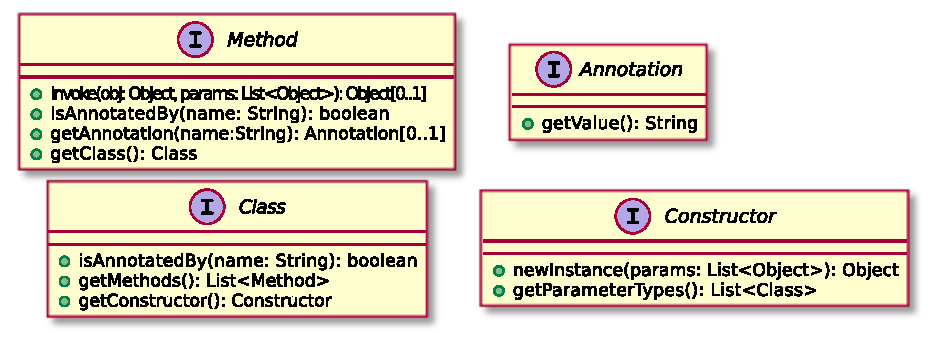
\includegraphics{diag.pdf}%
\end{center}
}

% Les questions peuvent également être créées avec un environnement 'questionExamBlock'.
% Cela garantit que la question sera affichée sur la même page que le contenu de l'environnement.
% Par exemple, cela peut être utilisé pour éviter de démarrer une nouvelle page sur un ecnadré de réponse.
\begin{questionExamBlock}{\lipsum[5]}
	\answerExam[white]{1.5}{18}{1}
\end{questionExamBlock}

% Comme pour les questions ordinaires, il est possible de définir une étiquette sur un bloc 'questionExamBlock'.
\begin{questionExamBlock}[q.otherlabel]{\lipsum[6][1]}
	\answerExam[white]{1.5}{10}{1}
\end{questionExamBlock}

\textbf{Référence à \cref{q.otherlabel}}


\end{document}
